\chapter{Arhitektura i dizajn sustava}

		Arhitekturu sustava općenito (pa tako i našeg) možemo podijeliti na tri dijela:
	\begin{itemize}
		\item 	\textit{Web poslužitelj}
		\item 	\textit{Web aplikacija}
		\item 	\textit{Baza podataka}		
	\end{itemize}
	
	\textbf{Internetski preglednik (web preglednik, web browser)} je dio arhitekture koji korisniku omogućuje pregled web-stranica pa tako i samoga sadržaja koji se nalazi na njoj. Korisnik putem web preglednika šalje HTTP zahtjev poslužitelju za dohvat željenog sadržaja i čeka HTTP odgovor. HTTP je protokol bez stanja što znači da primatelj ne smije zadržati stanje sesije iz prethodnih zahtjeva. Neki od popularnijih web preglednika su "Google Chrome" ili "Opera".
	
	\textbf{Web poslužitelj} je osnova svake web aplikacije. On šalje klijentu HTTP odgovor na određeni HTTP zahtjev. Korisnik koristi web aplikaciju na način da web aplikacija obrađuje zahtjev te ovisno o potrebi pristupa bazi podataka. Poslužitelj vraća odgovor u obliku HTML dokumenta koji je vidljiv korisniku.
		
    \begin{figure}[H]
    	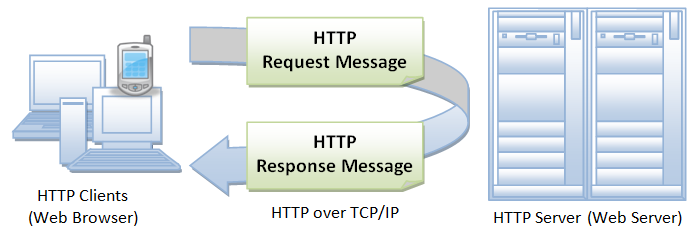
\includegraphics[scale=1.2]{slike/HTTP.PNG} %veličina slike u odnosu na originalnu datoteku i pozicija slike
    	\centering
    	\caption{Prikaz HTTP komunikacije između klijenta i poslužitelja}
    	\label{fig:promjene}
    \end{figure}
    
    \textit{\newline \newline}
    
    Naša grupa je za projekt na predmetu Programsko inženjerstvo (ak.god. 2023./2024.) odabrala React sustav za potrebe frontenda. Odabrali smo React zbog njegove jednostavne i moćne arhitekture koja omogućuje brz i održiv razvoj web aplikacija. React se temelji na principu komponenata, što znači da aplikaciju gradimo kao skup neovisnih dijelova sučelja, svaki s vlastitom logikom i stilovima. Time svaka komponenta postaje ponovno upotrebljiva i lako zamjenjiva što olakšava razvoj aplikacije.
    
    Za backend smo odabrali raditi u programskom jeziku Java i to u Spring Boot-u. Koristili smo Maven alat za izgradnju programskog koda. Spring Boot nam se svidio zbog dvije karakteristike: inverzija kontrole gdje sam Spring Boot kontrolira izvršavanje programskog koda te injektiranje objekata o kojima ovisi rad koda. Neke od karakteristika Spring Boot-a su: unaprijed pripremljene funkcionalnosti, nema generiranja klasa i koda već se koriste unaprijed definirane biblioteke. U svakom slučaju Spring Boot zna dosta olakšati programeru posao. Također olakšava i spajanje na bazu podataka o kojoj će biti više riječi u sljedećoj cjelini.
    
    Razvojno okruženje koje smo koristili zavisilo je od člana do člana ekipe, neki su radili u Eclipse-u, neki u IntelliJ. Koristili smo GitHub sustav za upravljanje verzijama programske potpore te TeXstudio za pisanje dokumentacije.
    
    \begin{figure}[H]
    	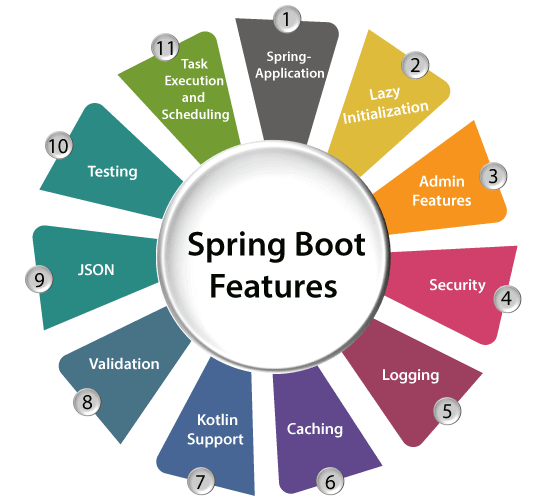
\includegraphics[scale=0.5]{slike/SpringBoot.PNG} %veličina slike u odnosu na originalnu datoteku i pozicija slike
    	\centering
    	\caption{Neke od koristi Spring Boot-a}
    	\label{fig:promjene}
    \end{figure}
		

				
	\section{Baza podataka}
			
		\hspace*{2em}
     	Za bazu podataka odabrali smo SQL vrstu baze podataka, točnije MySql software zbog svoje jednostavnosti i kvalitetne usluge. MySql je besplatni open-source sistem za upravljanje bazama podataka. Također ga podržava velika i aktivna zajednica korisnika što nam omogućava brz pronalazak potrebnih resursa, tutorijala i rješenja za moguće probleme. Što se performanse tiče, MySql je poznat po brzini i efikasnosti te se koristi kako za manje web aplikacije tako i za velike poslovne sisteme. Lako se integrira u različite programske jezike i razvojne okoline.
     	
     	\begin{figure}[H]
     		
\includegraphics[scale=1]{slike/MySql.PNG} %veličina slike u odnosu na originalnu datoteku i pozicija slike
     		\centering
     		\caption{MySql}
     		\label{fig:promjene}
     	\end{figure}
     	
		
		
			\subsection{Opis tablica}
			
				
				\hspace*{2em}
				Glavni cilj: Baza podataka osigurava pregled i pohranu podataka o svim faktorima procesa zauzimanja termina u medicinsko rehabilitacijskoj klinici. Kako bi se osiguralo pravilno rukovanje bazom podataka potrebne su pojedine tablice tj. entiteti od kojih svaki sadrži svoje atribute te odnose među pojedinim entitetima koji se u struci nazivaju „relationships“. Entiteti: Našu bazu podataka tvori nekoliko entiteta, preciznije: User (korisnik), Appointment (dogovoreni sastanak), Equipment (oprema) te Room (prostorija/radna sala). 
				\newline
				\hspace*{2em}
				Entitet User: To je najbitniji entitet jer sadrži podatke o svim djelatnicima medicinsko rehabilitacijske klinike, pacijentima i ostalim djelatnicima. Za ostvarivanje funkcionalnosti potrebni su sljedeći atributi: idUser(primary key), imeUser, prezime, oib, username, password, email, datum rođenja, spol, start date(unosi se pri stvaranju tj. kad je napravljen korisnički račun) te na kraju enum koji specijalizira entitet Usera na jedno od dvije opcije. To su Patient ili Employee. Employee-u se dalje bilježi status, tj. gleda li se na njega kao aktivnog zaposlenika, neaktivnog ili admin.
				\newline
				\hspace*{2em}
				Entitet Appointment: Entitet Appointment prikazuje sve dogovorene sastanke te omogućava uspješno dogovaranje novih bez da dođe do nekih problema kao što su kolizije ili nedostatak opreme. Atributi u entitetu Appointment su: idApp(primary key), vrijeme termina (od kad do kad je zakazan termin), user, opis termina, oprema i prostorija. 
				\newline
				\hspace*{2em}
				Entitet Equipment: Entitet Equipment sadrži podatke o svoj opremi. Osigurava da ne dođe do problema rezerviranja više opreme nego što je dostupno, na primjer pacijent A je rezervirao zadnje štake te pacijent B u istom terminu nema pristup tom komadu opreme. Atributi koji čine entitet Equipment su: idEqu(primary key), ime, opis i status(radi li ili ne). 
				\newline
				\hspace*{2em}
				Entitet Prostorija: Entitet Prostorija prikazuje podatke o mogućim prostorijama za rehabilitaciju. Osigurava da određena prostorija ne može biti zauzeta više puta odjednom. Atributi koji sačinjavaju entitet Prostorija su: idPro(primary key), ime i kapacitet. 
				\newline
				\hspace*{2em}
				Veze (relationships) među entitetima: Veze među entitetima osiguravanju pravilnu i predviđenu funkcionalnost cijelog sustava (web aplikacije), povezuju sve entitete na način koji tvori logiku povezanosti. Uspostavljene su tri veze u našoj bazi podataka: User  Appointment. Veza User - Appointment je one to many(jedan na više, 1 - N) tip veze. Jedan User može zatražiti više sastanaka. Appointment - Prostorija. Veza Appointment  Prostorija je one to many(jedan na više, 1 - N) tip veze. Više sastanaka se može održavati u isto vrijeme u istoj prostoriji. Prostorija - Equipment. Veza Prostorija  Equipment je one to many(jedan na više, 1 - N) tip veze. Više opreme se može držati u jednoj prostoriji.
				
				
				\begin{longtblr}[
					label=none,
					entry=none
					]{
						width = \textwidth,
						colspec={|X[2,l]|X[3.5,l]|X[6,l]|}, 
						rowhead = 1,
					}
					\hline \SetCell[c=3]{c}{\textbf{korisnik - User tablica}} \\ \hline[3pt]
					\SetCell{LightGreen}idUser & INT AUTO\_INCREMENT & Jedinstveni identifikator korisnika \\ \hline
					imeUser & VARCHAR(255) & Ime korisnika \\ \hline
					prezime & VARCHAR(255) & Prezime korisnika \\ \hline
					oib & INT & OIB korisnika \\ \hline
					username & VARCHAR(255) & Korisničko ime \\ \hline
					password & VARCHAR(255) & Lozinka \\ \hline
					datumRodenja & DATE & Datum rođenja \\ \hline
					spol & VARCHAR(1) & Spol (M ili F) \\ \hline
					startDate & DATE & Datum početka korisničkog računa \\ \hline
					email & VARCHAR(255) & E-mail adresa \\ \hline
				\end{longtblr}
				
				
				\begin{longtblr}[
					label=none,
					entry=none
					]{
						width = \textwidth,
						colspec={|X[2.5,l]|X[3.5,l]|X[6,l]|}, 
						rowhead = 1,
					}
					\hline \SetCell[c=3]{c}{\textbf{prostorija - Prostorija tablica}} \\ \hline[3pt]
					\SetCell{LightGreen}idPro & INT AUTO\_INCREMENT & Jedinstveni identifikator prostorije \\ \hline
					imePro & VARCHAR(255) & Ime prostorije \\ \hline
					kapacitet & INT & Kapacitet prostorije \\ \hline
				\end{longtblr}
				
				
				\begin{longtblr}[
					label=none,
					entry=none
					]{
						width = \textwidth,
						colspec={|X[2.5,l]|X[3.5,l]|X[6,l]|}, 
						rowhead = 1,
					}
					\hline \SetCell[c=3]{c}{\textbf{patient - Patient tablica}} \\ \hline[3pt]
					\SetCell{LightGreen}idUser & INT AUTO\_INCREMENT & Jedinstveni identifikator pacijenta \\ \hline
				\end{longtblr}
				
				
				\begin{longtblr}[
					label=none,
					entry=none
					]{
						width = \textwidth,
						colspec={|X[2.5,l]|X[3.5,l]|X[6,l]|}, 
						rowhead = 1,
					}
					\hline \SetCell[c=3]{c}{\textbf{employee - Employee tablica}} \\ \hline[3pt]
					\SetCell{LightGreen}statusEmp & VARCHAR(255) & Status zaposlenika \\ \hline
					idUser & INT AUTO\_INCREMENT & Jedinstveni identifikator zaposlenika \\ \hline
				\end{longtblr}
				
				
				\begin{longtblr}[
					label=none,
					entry=none
					]{
						width = \textwidth,
						colspec={|X[2.5,l]|X[3.5,l]|X[6,l]|}, 
						rowhead = 1,
					}
					\hline \SetCell[c=3]{c}{\textbf{appointment - Appointment tablica}} \\ \hline[3pt]
					\SetCell{LightGreen}idApp & INT AUTO\_INCREMENT & Jedinstveni identifikator termina \\ \hline
					vrijemeTermina & DATETIME & Vrijeme termina \\ \hline
					idUser & INT & Jedinstveni identifikator korisnika \\ \hline
					opisTermina & VARCHAR(255) & Opis termina \\ \hline
					idEqu & INT & Jedinstveni identifikator opreme \\ \hline
					idPro & INT & Jedinstveni identifikator prostorije \\ \hline
				\end{longtblr}
				
				
				\begin{longtblr}[
					label=none,
					entry=none
					]{
						width = \textwidth,
						colspec={|X[2.5,l]|X[3.5,l]|X[6,l]|}, 
						rowhead = 1,
					}
					\hline \SetCell[c=3]{c}{\textbf{equipment - Equipment tablica}} \\ \hline[3pt]
					\SetCell{LightGreen}idEqu & INT AUTO\_INCREMENT & Jedinstveni identifikator opreme \\ \hline
					imeEqu & VARCHAR(255) & Ime opreme \\ \hline
					opisEqu & VARCHAR(255) & Opis opreme \\ \hline
					statusEqu & VARCHAR(255) & Status opreme \\ \hline
					idPro & INT & Jedinstveni identifikator prostorije \\ \hline
				\end{longtblr}
				
			\newpage
			
			\subsection{Dijagram baze podataka}
				
				\begin{figure}[H]
					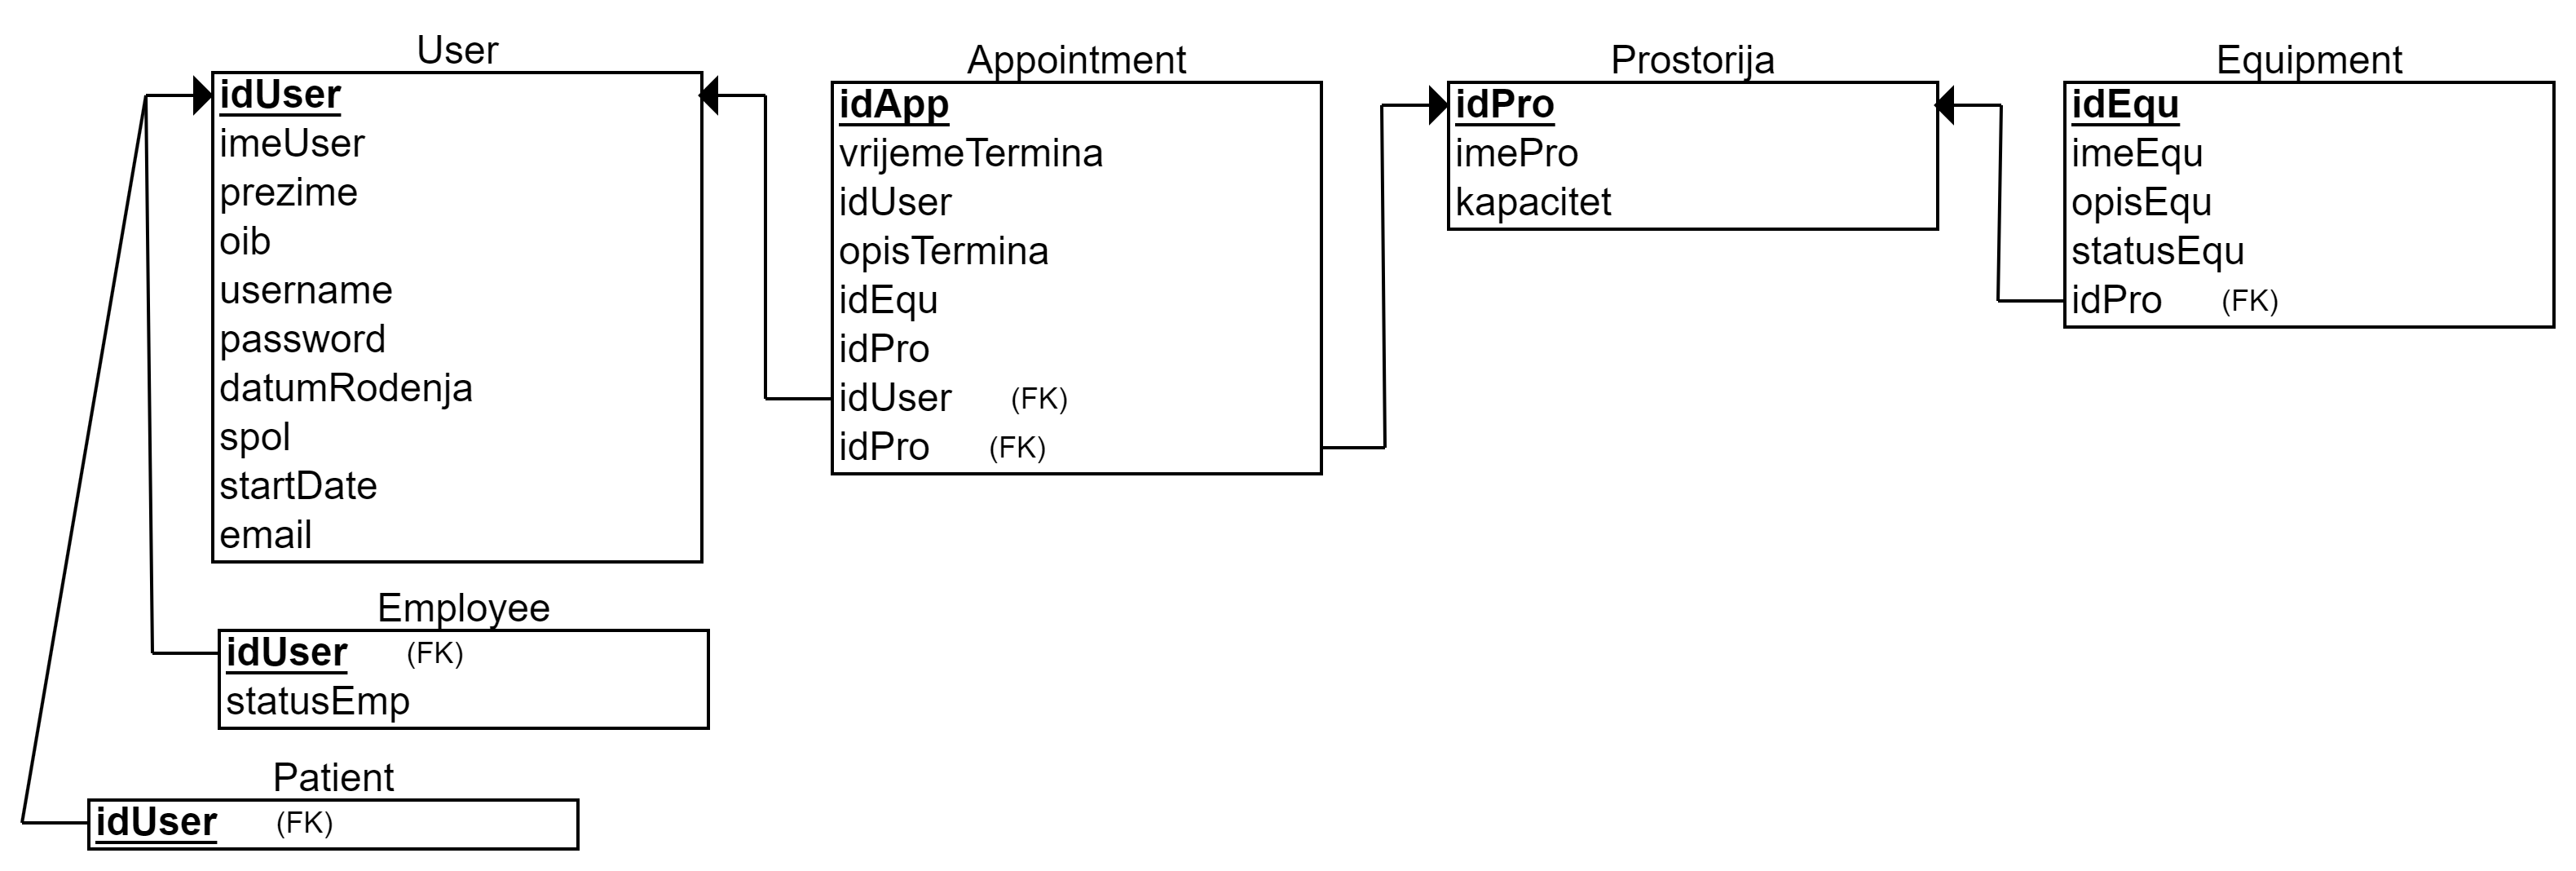
\includegraphics[scale=0.14]{slike/bp_rel.PNG} %veličina slike u odnosu na originalnu datoteku i pozicija slike
					\centering
					\caption{Relacijski model baze podataka}
					\label{fig:promjene}
				\end{figure}
				
				\begin{figure}[H]
					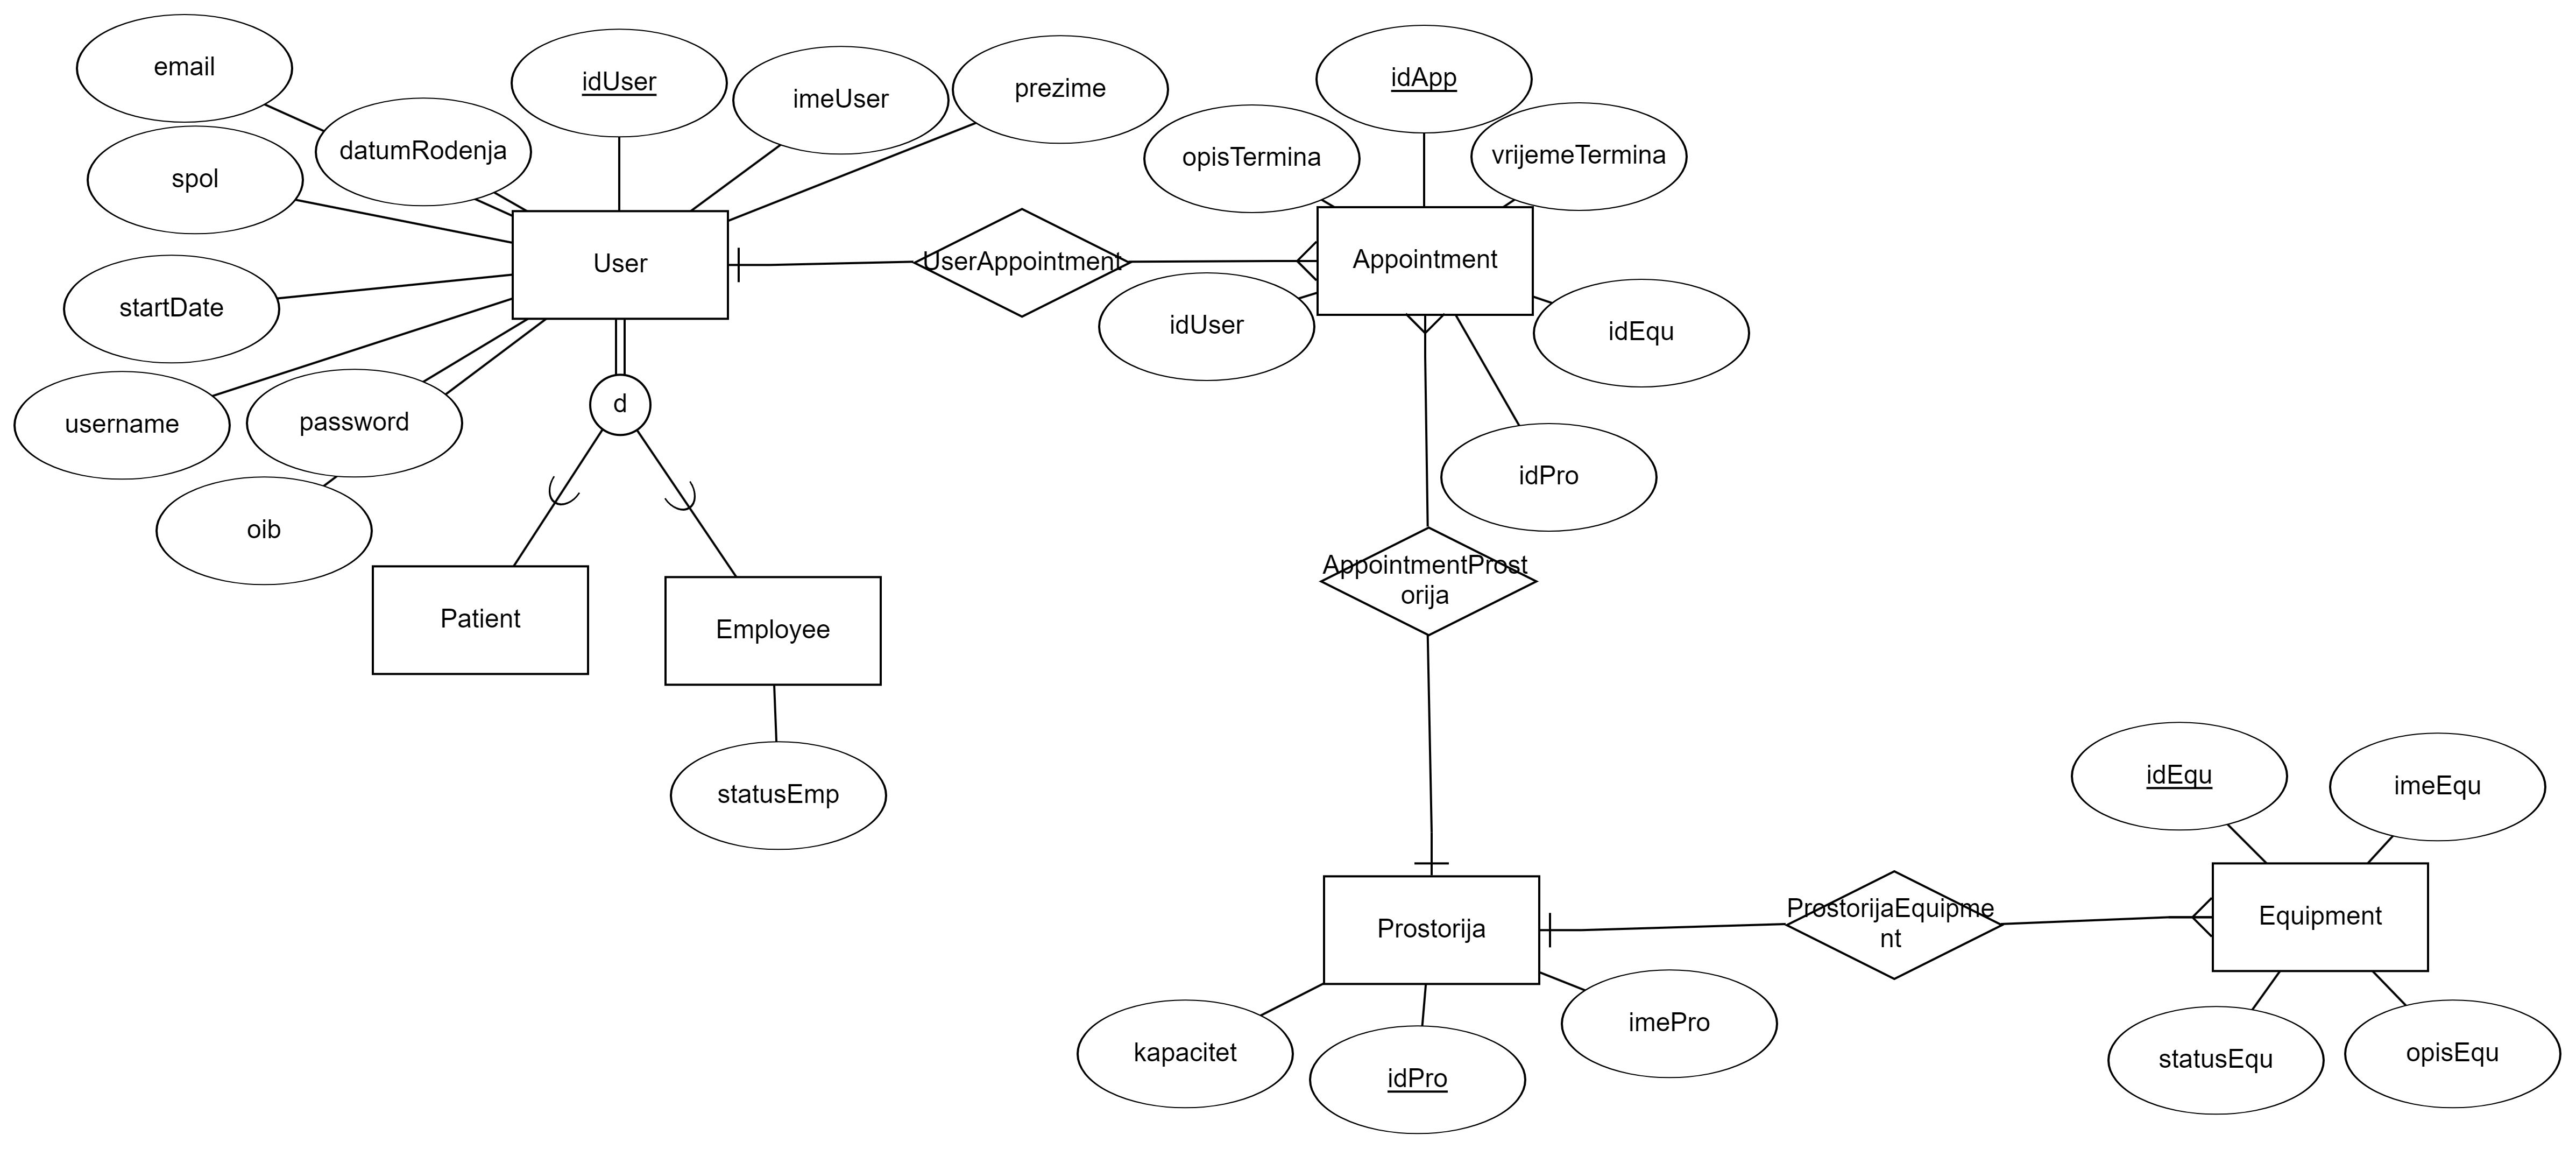
\includegraphics[scale=0.085]{slike/bp_er.PNG} %veličina slike u odnosu na originalnu datoteku i pozicija slike
					\centering
					\caption{ER model baze podataka}
					\label{fig:promjene}
				\end{figure}
			
			\eject
			
			
		\section{Dijagram razreda}
		
			Na slici 4.6 prikazani su razredi kojima se predstavlja struktura baze podataka u našoj aplikaciji te su razredi User, Appointment, Room, Schedule i Equipment entiteti u bazi podataka. Implementirane metode služe za komunikaciju s bazom podataka te po potrebi izvršavaju pisanje, brisanje ili dohvaćanje podataka iz same baze. Razred User predstavlja svakog korisnika aplikacije. Kako bi korisnik mogao upotrebljavati pogodnosti koje aplikacija nudi, on se najprije mora registrirati u sustav koristeći osobne podatke: ime, prezime, korisničko ime, lozinka, email, OIB, spol te datum rođenja. Razred User također koristi i enumeraciju Role koja predstavlja ulogu korisnika u sustavu. Razred User također može zakazati i otkazati termin terapije, koju predstavlja razred Appointment. Razred Appointment sadrži podatke o samome terminu terapije te ga samo korisnici s pripadajućom ulogom EMPLOYEE, ADMINEMPLOYEE mogu otkazati ili stvoriti. Entitet Schedule koristi se prilikom stvaranja, odnosno potvrde samoga termina. Svrha je zauzimanje termina po datumima i satima s pripadajućom prostorijom za pregled te opremom za pregled, što omogućava provjeru raspoloživosti određenog datuma, vremena, sobe te opreme. Entitet Room koristi se za spremanje podataka o svakoj prostoriji ustanove te njih u sustav dodaje korisnik s ulogom ADMIN. ADMIN također jedini barata funkcijama vezanim za uređivanje atributa prostorija. Entitet Equipment predstavlja opremu koja se koristi prilikom medicinske rehabilitacije. Oprema je vezana uz određenu prostoriju te ju također zadaje ADMIN.
		
			\begin{figure}[H]
				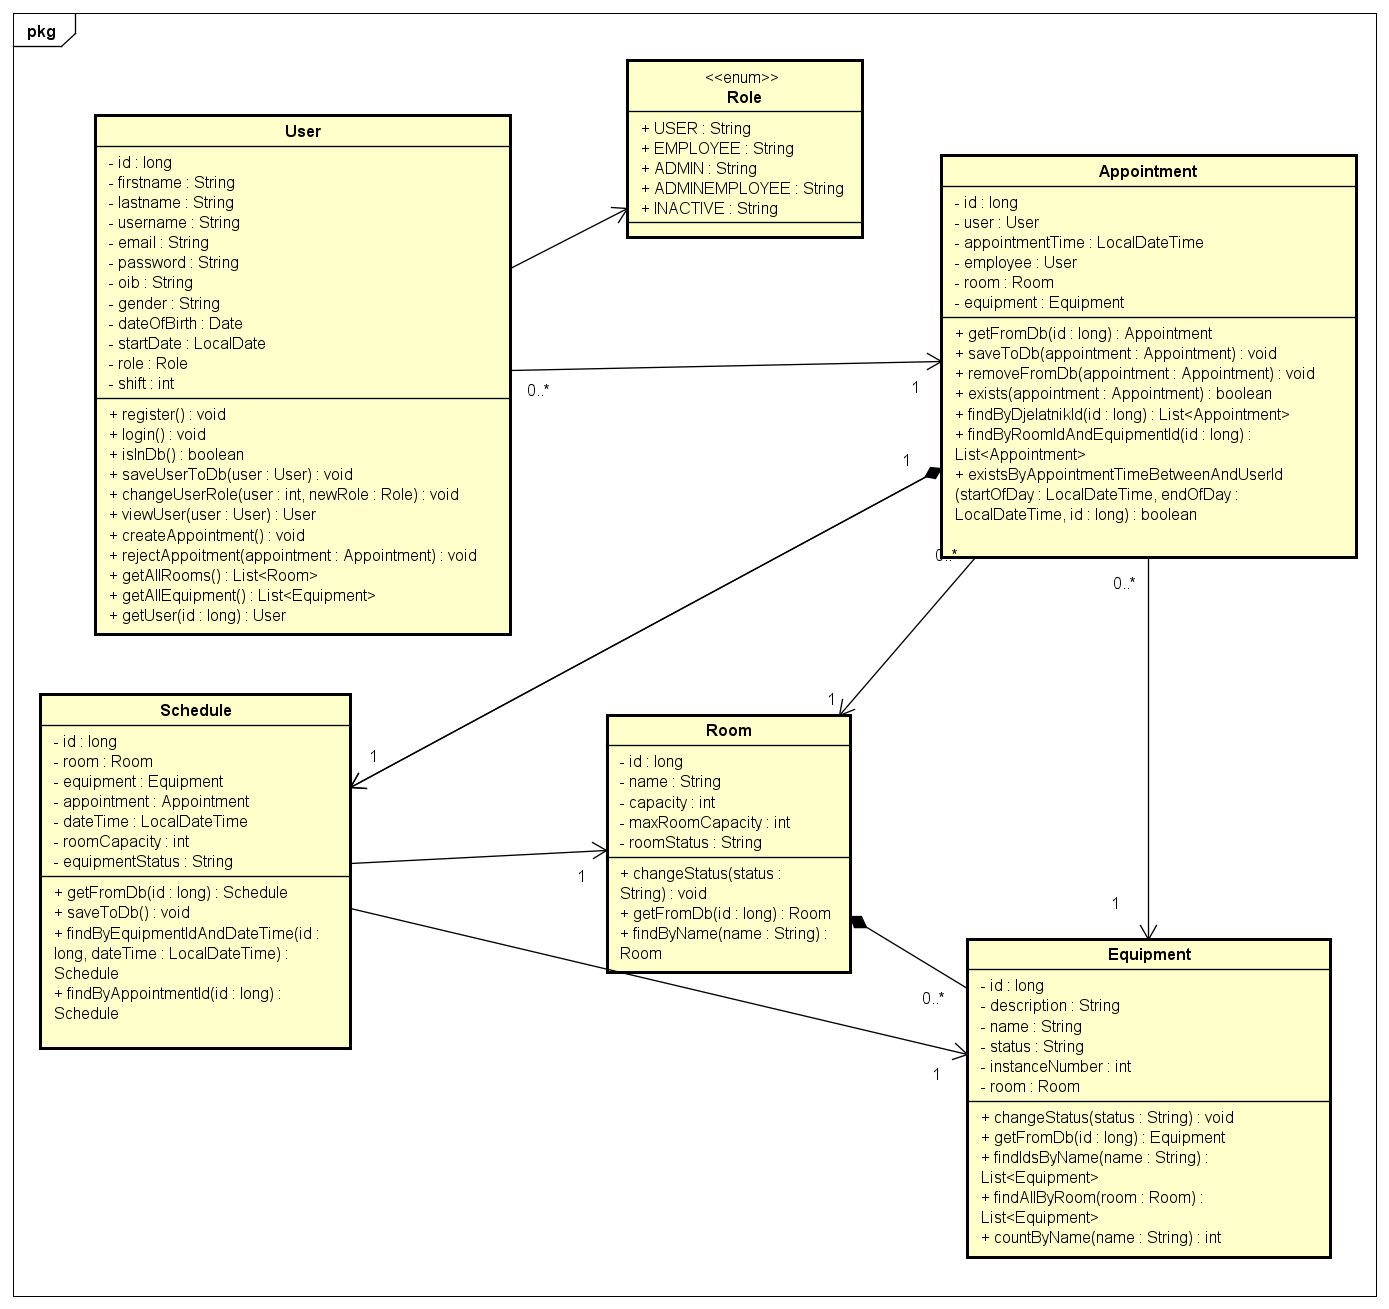
\includegraphics[scale=0.45]{slike/modeli_v2}
				\centering
				\caption{Dijagram razreda - Modeli}
			\end{figure}
			
			\newpage
			
			Na slici 4.7 prikazani su razredi kojima se povezuje Backend i Frontend dio same aplikacije. Razred AuthenticationController bavi se adekvatnom provjerom informacija koje korisnik unosi te omogućava njegovu registraciju, autentikaciju, izmjenu osobnih podataka poput lozinke, korisničkog imena ili emaila ako ih je zaboravio. Razred AdminController omogućava Adminu da dodaje nove zaposlenike, uklanja ljude s kojima više nema radnog odnosa, dobiva popis svih zaposlenika, dodaje i dohvaća prostorija, opreme te izmjena njihovih parametara. Razred AppController služi za povezivanje s frontend dijelom aplikacije i prikazivanje odabranih stranica, npr. stranica za registraciju, stranica za prijavu te provjerava valjanost podataka prilikom prijave i registracije. UserController se bavi korisnikom koji ima ulogu USER te omogućava dohvat svih korisnikovih zakazanih termina, dohvat prijašnjih opisa fizikalnih problema, te slanje i poništavanje zahtjeva za terminom. EmployeeController koriste korisnici s ulogama EMPLOYEE i ADMINEMPLOYEE te on služi za obradu zahtjeva za terminom - njihovo prihvaćanje, odbijanje, brisanje i izmjena određenih parametara.
			
			\begin{figure}[H]
				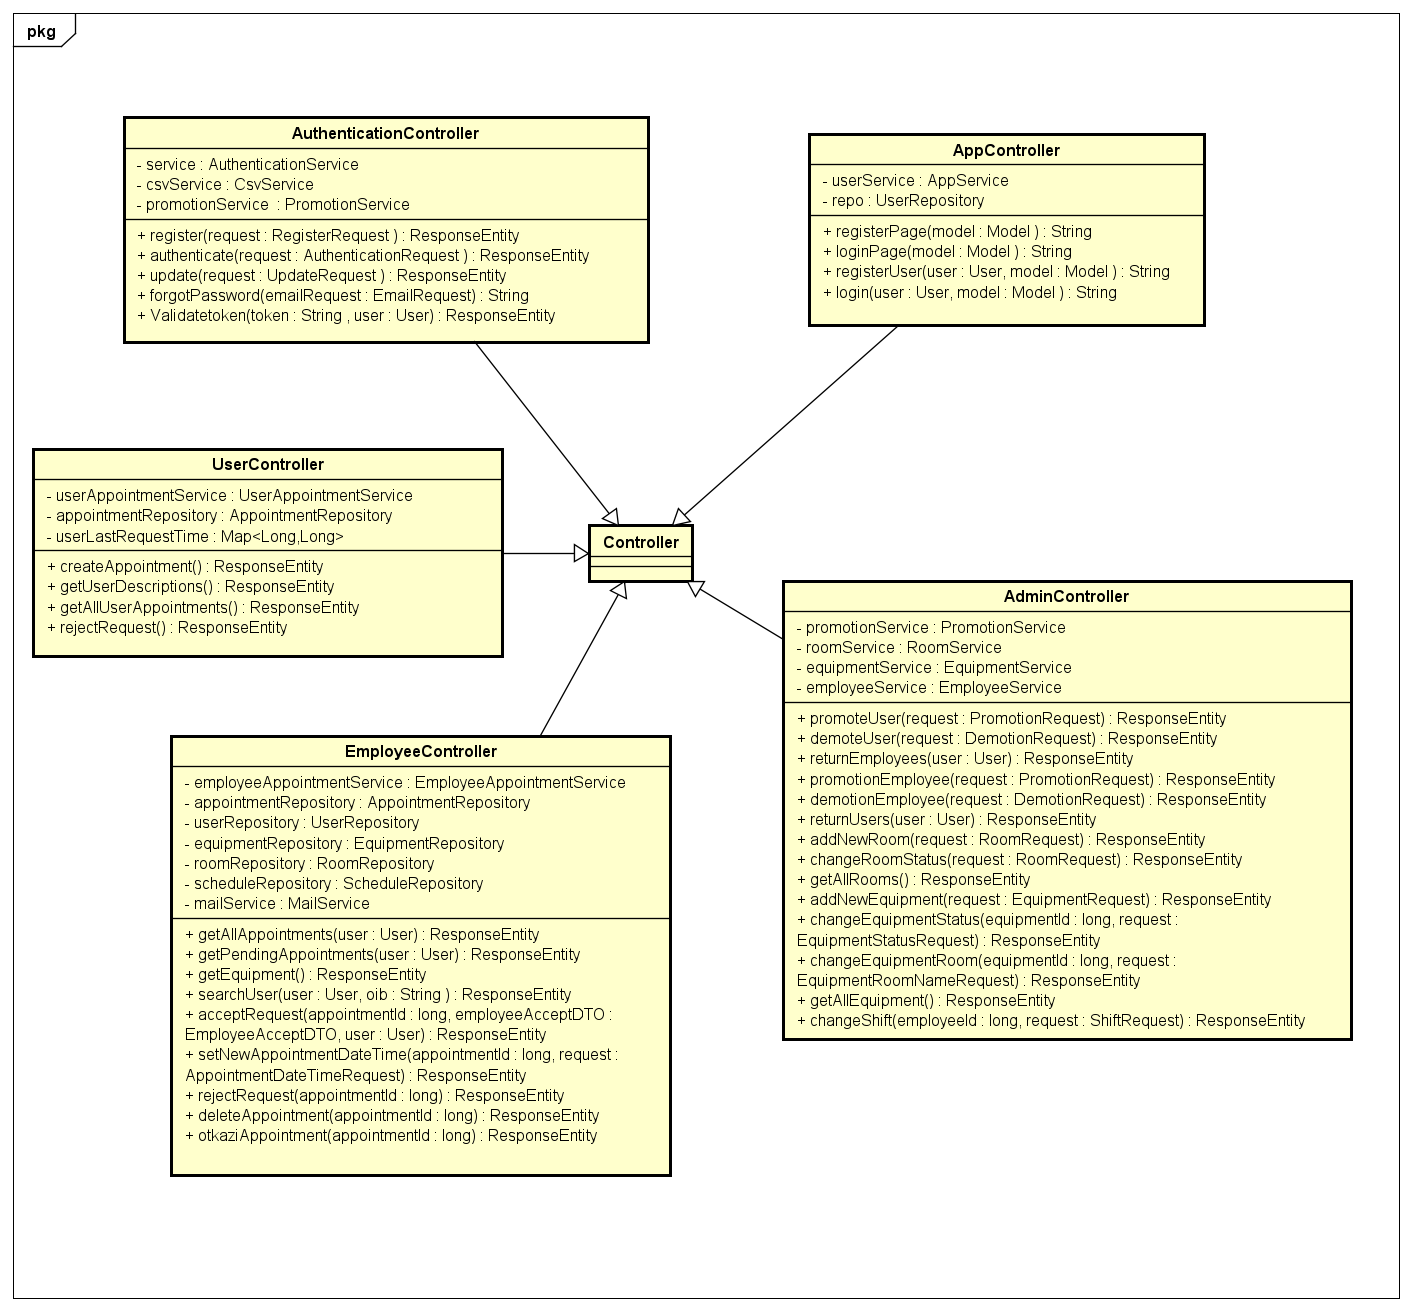
\includegraphics[scale=0.45]{slike/kontroleri_v2}
				\centering
				\caption{Dijagram razreda - Kontroleri}
			\end{figure}
			
			
			\textbf{\textit{dio 2. revizije}}\\			
			
			\textit{Prilikom druge predaje projekta dijagram razreda i opisi moraju odgovarati stvarnom stanju implementacije}
			
			
			
			\eject
		
		\section{Dijagram stanja}
			
			
		\begin{figure}[H]
			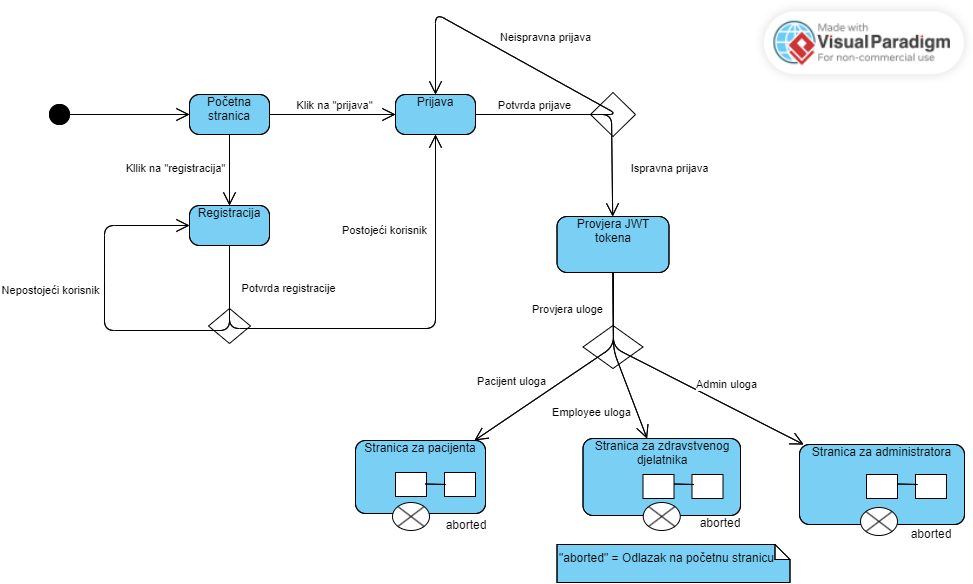
\includegraphics[scale=0.4]{slike/DijagramStanja1.PNG} %veličina slike u odnosu na originalnu datoteku i pozicija slike
			\centering
			\caption{Dijagram stanja početne stranice}
			\label{fig:promjene}
		\end{figure}
		
			\begin{figure}[H]
			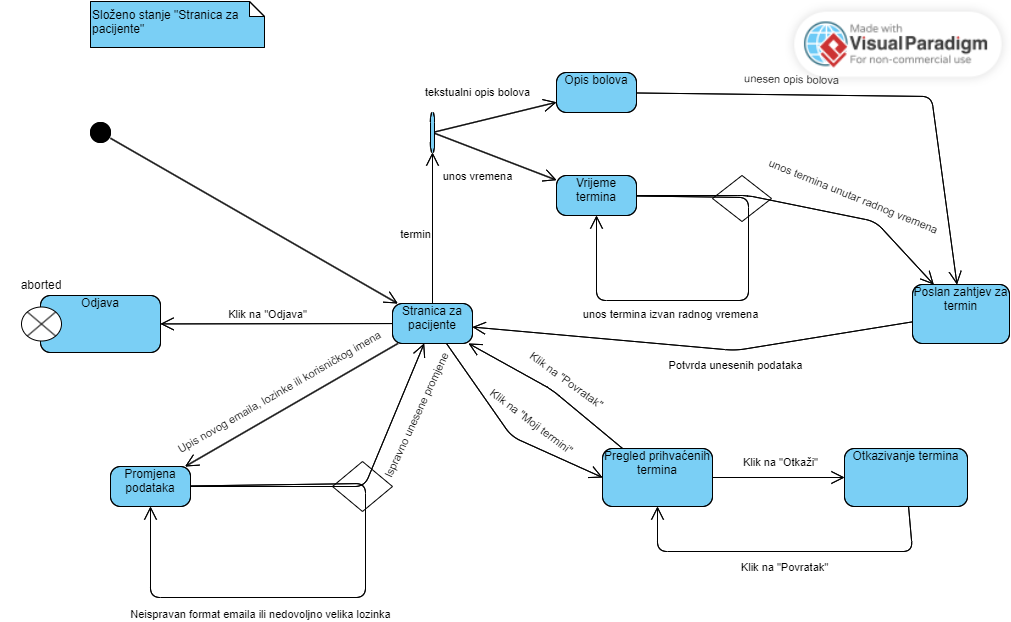
\includegraphics[scale=0.4]{slike/DijagramStanja2.PNG} %veličina slike u odnosu na originalnu datoteku i pozicija slike
			\centering
			\caption{Složeno stanje "Stranica za pacijenta"}
			\label{fig:promjene}
		\end{figure}
		
		\begin{figure}[H]
			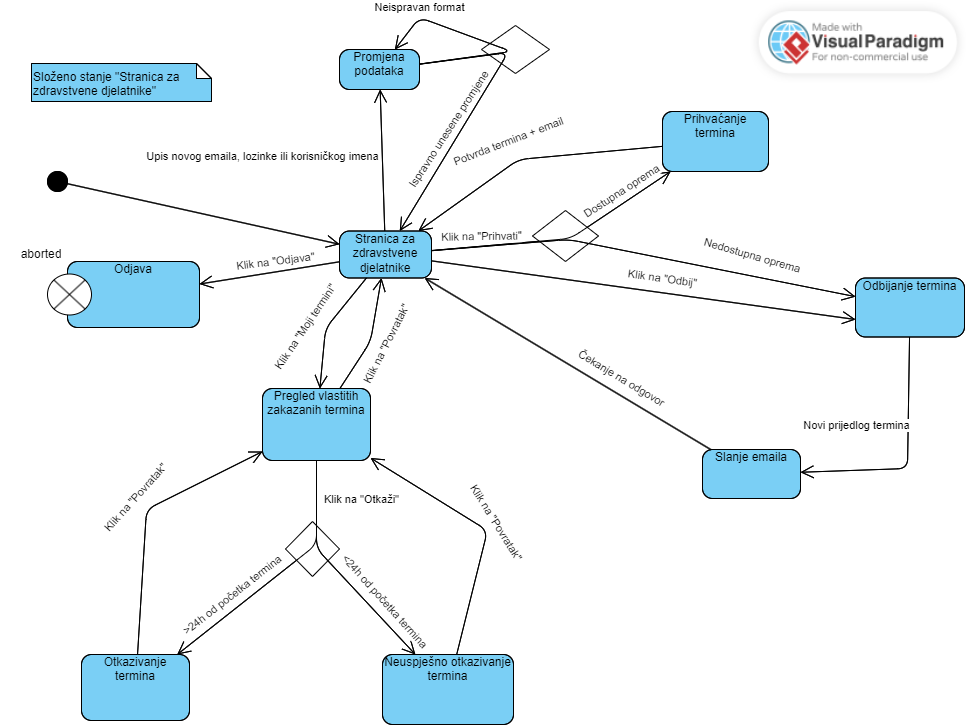
\includegraphics[scale=0.5]{slike/DijagramStanja3.PNG} %veličina slike u odnosu na originalnu datoteku i pozicija slike
			\centering
			\caption{Složeno stanje "Stranica za zdravstvenog djelatnika"}
			\label{fig:promjene}
		\end{figure}
		
		Složeno stanje "Stranica za adminemployee" je vrlo slična složenom stanju "Stranica za zdravstvenog djelatnika" uz još dodatnu mogućnost dodavanje opreme i soba. Iz tog razloga smatramo da nije potrebno postaviti i taj dijagram stanja (jer je to kombinacija stanja iz složenog stanja "Stranica za zdravstvenog djelatnika" i "Stranica za administratora").
			
				\begin{figure}[H]
				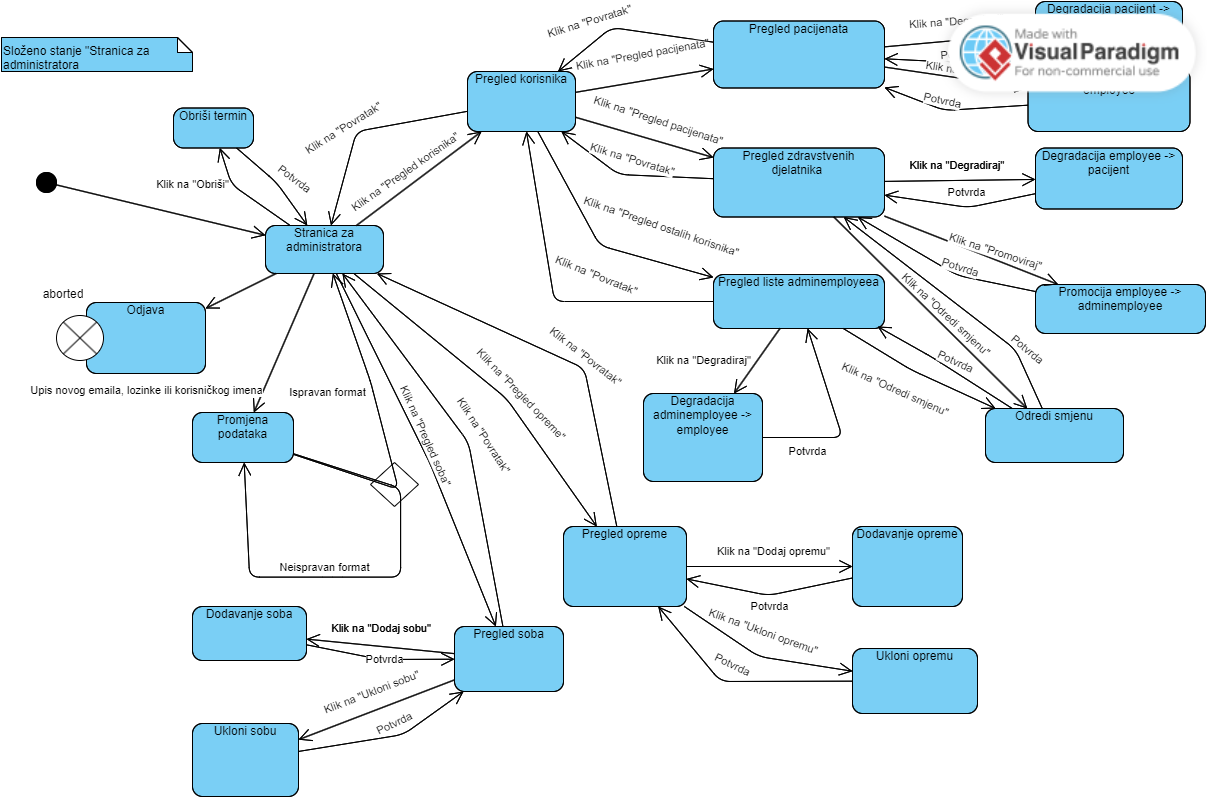
\includegraphics[scale=0.4]{slike/DijagramStanja4.PNG} %veličina slike u odnosu na originalnu datoteku i pozicija slike
				\centering
				\caption{Složeno stanje "Stranica za administratora"}
				\label{fig:promjene}
			\end{figure}
			
			\eject
			
		\section{Dijagram aktivnosti}
			
			\begin{figure}[H]
				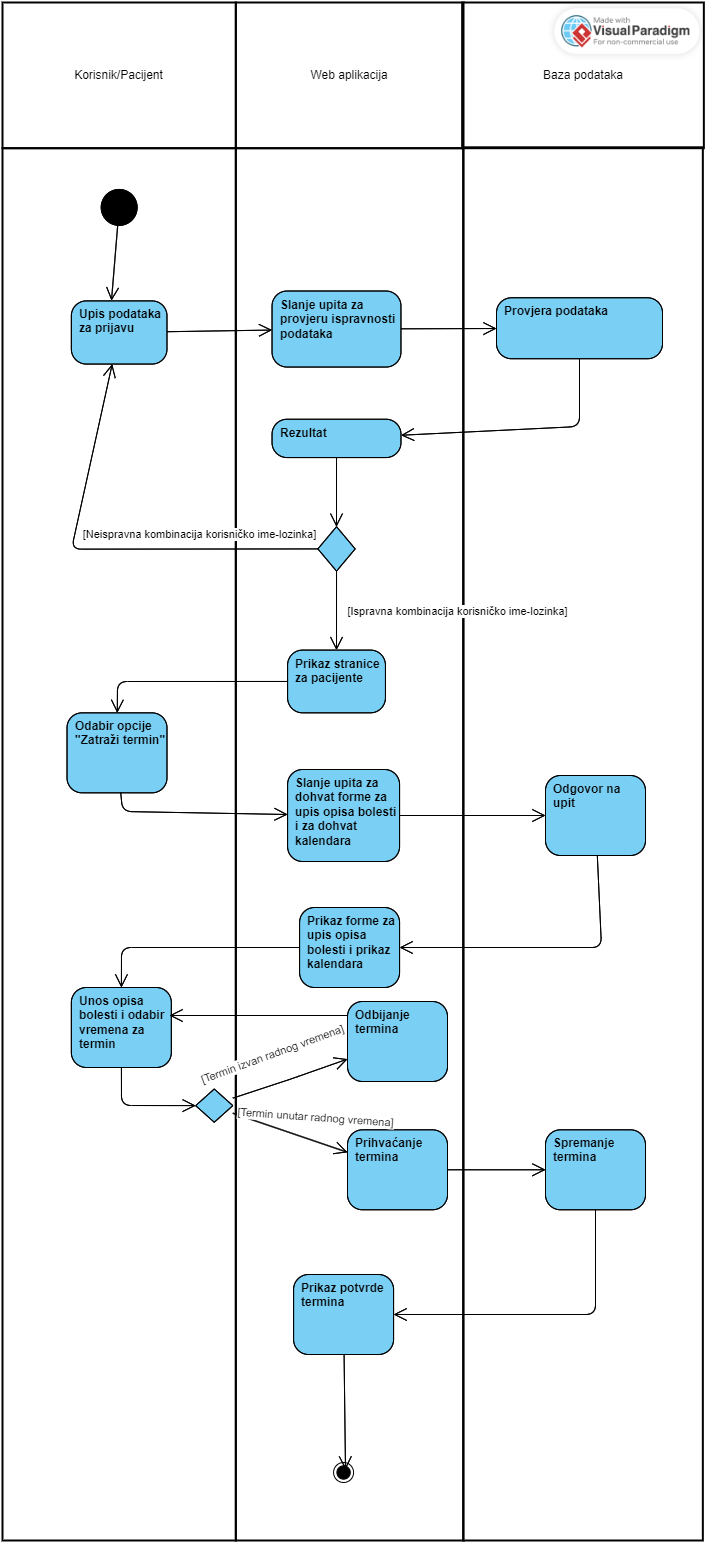
\includegraphics[scale=0.35]{slike/DijagramAktivnosti1.PNG} %veličina slike u odnosu na originalnu datoteku i pozicija slike
				\centering
				\caption{Prikaz dijagrama aktivnosti pri zahtjevu za novi termin}
				\label{fig:promjene}
			\end{figure}
			
			\begin{figure}[H]
				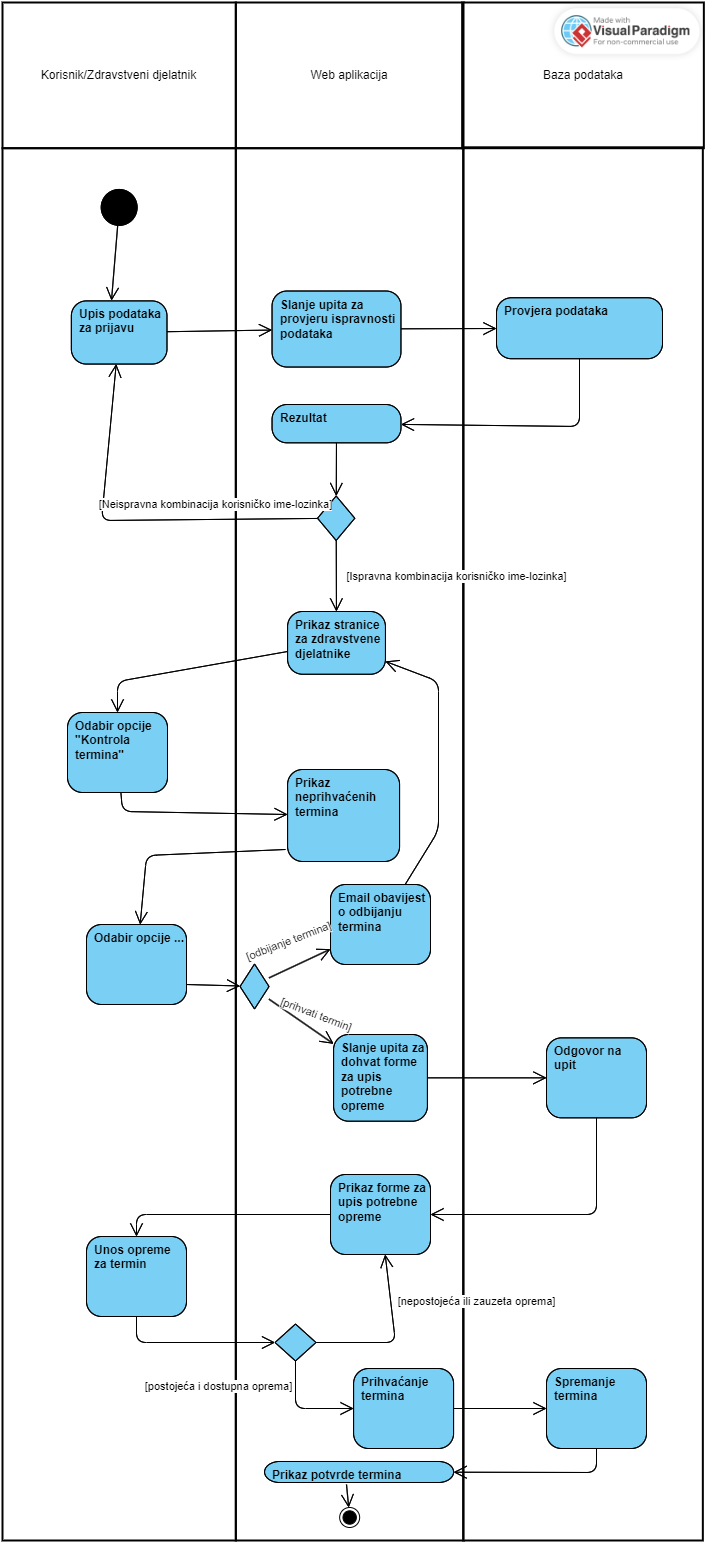
\includegraphics[scale=0.35]{slike/DijagramAktivnosti2.PNG} %veličina slike u odnosu na originalnu datoteku i pozicija slike
				\centering
				\caption{Prikaz dijagrama aktivnosti pri potvrđivanju/odbijanju termina}
				\label{fig:promjene}
			\end{figure}
			
			\begin{figure}[H]
				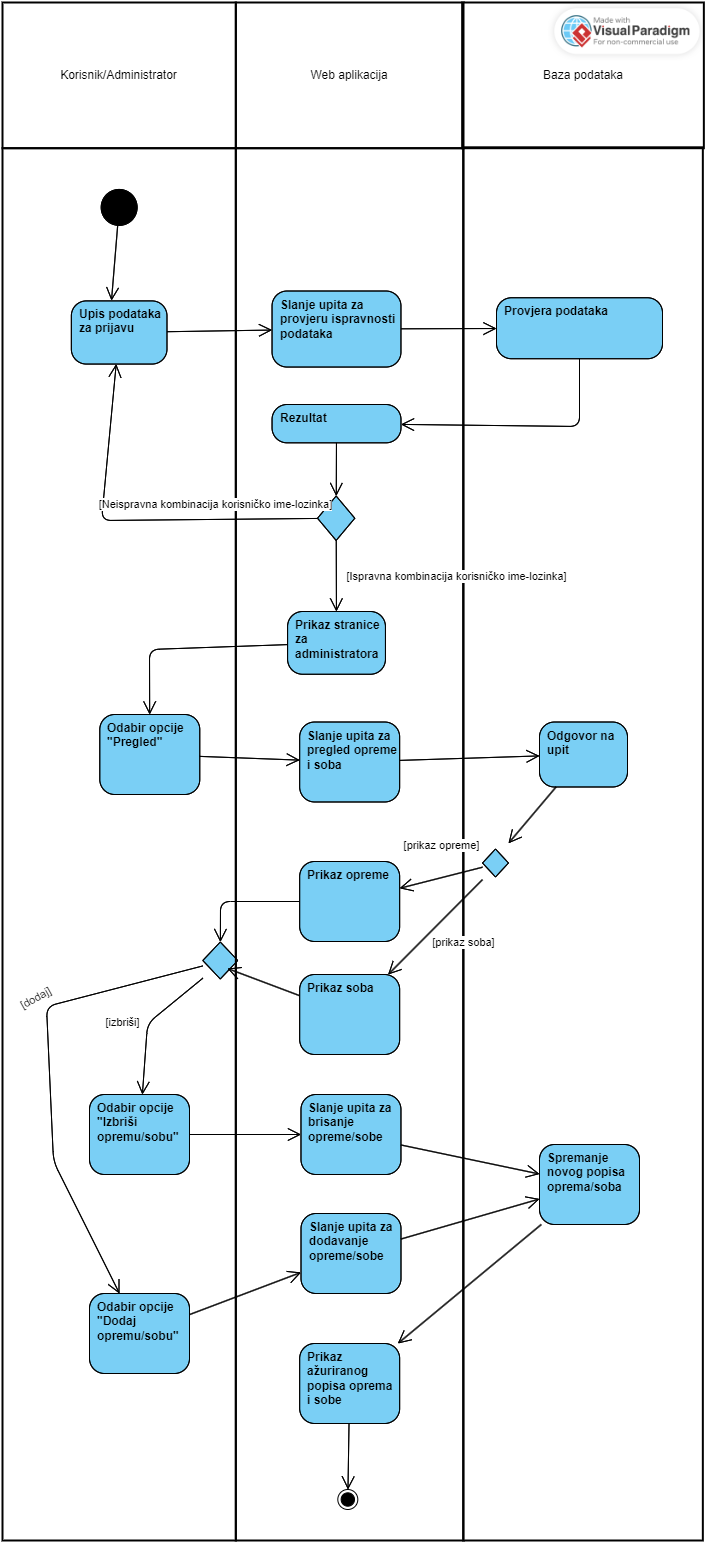
\includegraphics[scale=0.35]{slike/DijagramAktivnosti3.PNG} %veličina slike u odnosu na originalnu datoteku i pozicija slike
				\centering
				\caption{Prikaz dijagrama aktivnosti pri dodavanju soba/opreme}
				\label{fig:promjene}
			\end{figure}
			
			\eject
		\section{Dijagram komponenti}
		
			\begin{figure}[H]
				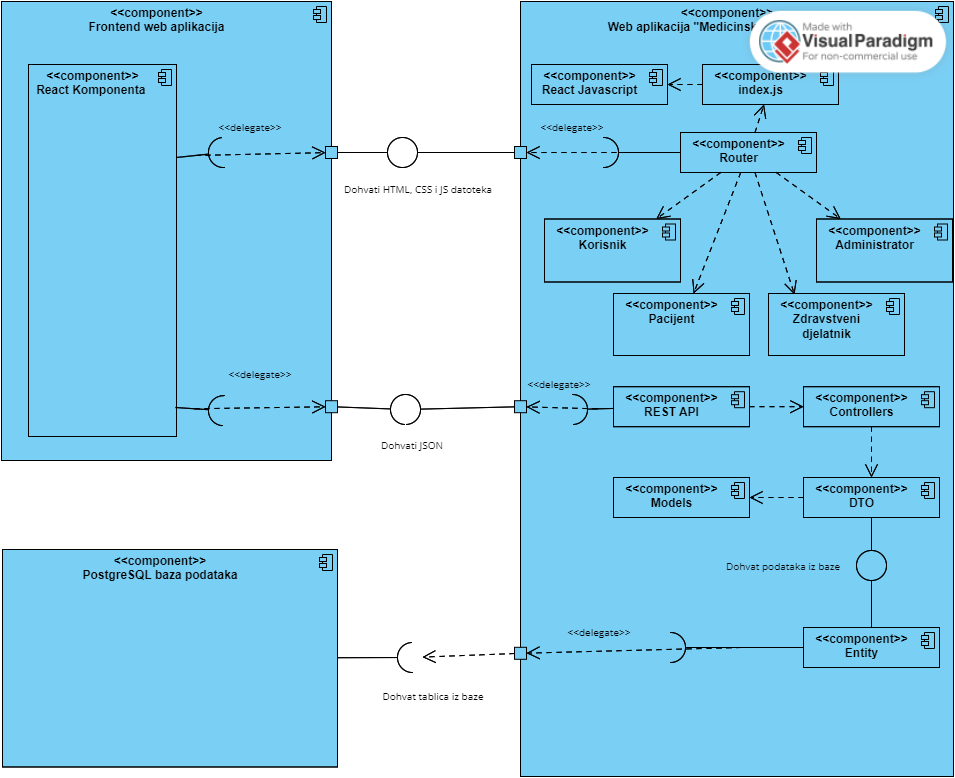
\includegraphics[scale=0.52]{slike/DijagramKomponenti.PNG} %veličina slike u odnosu na originalnu datoteku i pozicija slike
				\centering
				\caption{Prikaz dijagrama komponenti naše web aplikacije}
				\label{fig:promjene}
			\end{figure}